\documentclass[10pt,a4paper]{article}
\usepackage[T1]{fontenc}
\usepackage[utf8]{inputenc}
\usepackage[margin=22mm]{geometry}
\usepackage{lmodern,microtype,amsmath,amssymb,booktabs,tabularx,graphicx,float,xcolor}
\usepackage[font=small,labelfont=bf]{caption}
\usepackage[colorlinks=true,linkcolor=blue,citecolor=blue,urlcolor=blue]{hyperref}
\usepackage{url}

\setlength{\parskip}{4pt}
\setlength{\parindent}{0pt}
\emergencystretch=2em
\newcommand{\CO}{CO\textsubscript{2}}
\title{Regime-Dependent Routing-Policy Preference:\\When Adapting an Established Routing Policy Pays, and When It Does Not}
\author{Author details to be supplied}
\date{Conference submission draft --- 21 September 2026}
\begin{document}
\maketitle

\begin{abstract}
Navigation systems implement several established pre-trip routing objectives --- shortest distance, dynamic travel time, constrained eco-routing --- but the choice \emph{among} them is normally fixed by design rather than by traffic condition. We characterise that choice empirically. In 432 completed SUMO simulations over 24 controlled contexts on a 12-signal urban mesh, the preferred policy reverses with demand: shortest-distance routing is preferred in every low-demand context, dynamic travel-time routing in every high-demand context, and the reversal is displaced by the signal regime, crossing between 720 and 1200\,veh/h under balanced signals but only between 1200 and 1680\,veh/h under arterial-priority signals. The reversal is worth having: adapting the policy rather than fixing it removes 0.03018 units of mean decision regret against the best fixed policy, and a depth-3 regression tree predicting policy outcomes from pre-decision context recovers 79.9\% of that headroom under leave-one-context-out evaluation (mean regret 0.00606, 21/24 contexts optimal). The same selector is \emph{harmful} when the held-out context lies outside the demand range it was trained on: holding out an entire demand level, mean regret rises to 0.07649 against 0.03018 for the best fixed policy. Two audited negative controls bound the scope: an environmental routing objective collapsed onto shortest-distance routing (outcome-identical in 21/24 contexts; 21.62\% route-order selection loss) and was removed from the portfolio, and the preference weights left every selector decision unchanged across the full time-to-emissions range. Adaptive routing-policy selection is therefore governed by regime coverage of the context space, not by model capacity. We introduce no routing, decision or learning algorithm.
\end{abstract}
\textbf{Keywords:} routing-policy selection; traffic regimes; SUMO; decision regret; algorithm selection; eco-routing.

\section{Introduction}
Choosing a route and choosing a \emph{routing policy} are different decisions. A pre-trip planner may minimise distance, estimated travel time, or an estimated environmental cost; production navigation systems commit to one such objective and apply it uniformly. Whether that commitment costs anything, and under what conditions, is an empirical question about the traffic environment rather than about the planner.

This paper answers it for a controlled synthetic environment. Our question is:
\begin{quote}
\emph{Under what traffic regimes does the preferred routing policy change, how much decision value is available from adapting that policy, and how reliably can the resulting structure be identified on unseen and out-of-regime contexts?}
\end{quote}

The object of study is the mapping from observable pre-trip context to preferred established policy. A learned selector appears only as the instrument that tests whether that mapping is recoverable; it is not the contribution. We report four findings, each from completed simulation evidence.

\textbf{(1) Routing-policy preference is regime-structured.} Shortest-distance routing (SP) is preferred in all eight low-demand contexts and dynamic travel-time routing (DTT) in all eight high-demand contexts. The preference reverses monotonically in demand in every one of the eight restriction/signal cells.

\textbf{(2) The signal regime displaces the reversal.} Under balanced signal timing the reversal occurs between 720 and 1200\,veh/h in all four restriction configurations; under arterial-priority timing it occurs between 1200 and 1680\,veh/h in three of four. The signalisation plan, not only the demand, determines where policy adaptation begins to matter.

\textbf{(3) The headroom is real and largely recoverable.} Adapting the policy is worth 0.03018 mean additive regret units against the best fixed policy. A depth-3 regression tree recovers 79.9\% of it on held-out contexts.

\textbf{(4) There is an extrapolation boundary.} The same selector applied to an unseen demand regime is worse than simply fixing the best policy. The operative requirement is that training contexts span the regimes that will be met.

\textbf{Scope of the claim.} We claim no new routing algorithm, no new multi-criteria method and no new learning algorithm. The concepts we use --- context-aware route guidance, learned selection among algorithms, and multi-criteria evaluation of routing outcomes --- are all established, and Section~2 identifies the specific prior studies that establish them. What this paper supplies is an empirical measurement, on one controlled benchmark, of \emph{where} the preference between two established policies reverses, \emph{how much} that reversal is worth as a decision, and \emph{where the resulting adaptation stops being reliable}. Two prior negative results from the same project --- a failed environmental route-cost estimator and a preference layer that changes no decision --- are retained as audited controls that delimit what the positive findings mean rather than being removed from the record.

\textbf{Why this matters operationally.} A navigation operator choosing a single pre-trip objective is implicitly asserting that one objective dominates across the conditions its users encounter. Our pilot environment satisfied that assertion: one policy was best in all 30 contexts, so adaptation was worthless there. The present network does not, and the difference is not a property of the algorithms --- which are unchanged --- but of the traffic environment. Establishing which of the two situations one is in is therefore a measurement problem that precedes any decision to deploy an adaptive selector, and the last of our four findings shows that getting that measurement wrong in a specific way, by fitting outside the regimes that will actually be met, is worse than not adapting at all.

\section{Related work}
We position the study against seven established strands and then state what remains specific to this experiment. None of the seven is claimed as a contribution.

Shortest-path optimisation over additive link costs is the base case \cite{dijkstra1959note}, and minimising estimated travel time rather than distance is the standard dynamic variant. Both are long established and we implement them by enumeration over a finite catalogue of legal paths; neither the objectives nor their implementation is novel here.

\textbf{(2) Dynamic and traffic-informed routing.} A large literature improves route guidance by exploiting observed or predicted conditions: stochastic time-dependent routing policies \cite{gao2006optimal,levering2021framework}, proactive rerouting strategies that balance load across $k$ shortest paths \cite{pan2013proactive}, and real-time control formulations \cite{pi2017stochastic}. These works improve a routing mechanism. We hold the mechanisms fixed and study the choice between them, so their improvements are orthogonal to our question.

\textbf{(3) Environmental routing.} Eco-routing from historical and real-time information, vehicle emission prediction, and travel-time-constrained eco-routing all precede this work \cite{boriboonsomsin2012ecorouting,zeng2016prediction,zeng2017svm}; Huang and Peng compare shortest, fastest, eco and constrained-eco objectives using a soft time constraint \cite{huang2018ecorouting}. The four objective types are therefore not our contribution; we disclose the hard-filter adaptation of the constrained variant in Section~3.1. Our engagement with this strand is negative and is reported as such: in our environment the environmental objective did not yield a distinct policy (Section~4.4).

\textbf{(4) Context-aware routing and regime effects.} That routing-strategy performance depends on network load is established. Analytical work on non-Markovian routing dynamics derives distinct efficiency phases as a function of the mix between shortest-time and shortest-distance preference, showing that routing preference can move a system between qualitatively different regimes \cite{routing2026phase}. Falek~et~al.\ ask when real-time re-routing is worthwhile and find, from three months of city speed data, that it is seldom useful except during rush hours and for long routes \cite{falek2021reroute}. Novikov~et~al.\ study congestion thresholds for triggering dynamic re-routing \cite{novikov2018dynamic}. Chen~et~al.\ evaluate a load-aware detour strategy across a range of traffic densities \cite{chen2025detour}. Du~et~al.\ report that the advantage of learning-based over rule-based re-routing is itself regime-dependent \cite{du2023fogcloud}.

These studies establish demand dependence for a single adaptive mechanism, typically comparing re-routing against not re-routing, and mostly on abstract or analytical models. Context-aware route guidance is thus a mature idea and we do not claim it.

\textbf{(5) Algorithm and policy selection.} Rice's formulation of per-instance algorithm selection \cite{rice1976algorithm} and its modern instantiations \cite{bischl2016aslib,xu2008satzilla} map instance features to algorithm performance and select accordingly. Xie~et~al.\ already compare route-choice models in SUMO and discuss automatic selection and meta-learning \cite{xie2014unified}, so applying selection to routing is not proposed here as a new concept. Our use of this strand is methodological: it supplies the evaluation discipline --- per-instance scoring against a portfolio --- that we apply to routing policies.

\textbf{(6) From prediction to decision.} Predictive accuracy and decision quality need not coincide \cite{elmachtoub2022smart}. We use that distinction in two places: as the evaluation principle for the selector, which is scored by the quality of the policy it picks rather than by regression error; and as the diagnostic that condemned our environmental estimator, which had acceptable aggregate error but misordered routes. We do not adopt a decision-focused training loss, so the contribution of \cite{elmachtoub2022smart} is conceptual here, not algorithmic.

\textbf{(7) Regret and virtual-best benchmarks.} Opportunity loss against the best available alternative \cite{kouvelis1997robust} is the standard decision metric, and the algorithm-selection literature pairs it with a Virtual Best Solver: the retrospective selection of the best algorithm per instance, used to upper-bound what selection could achieve \cite{bischl2016aslib}. Our hindsight best-policy benchmark is the routing counterpart. Preference modelling --- additive value, TOPSIS, VIKOR, PROMETHEE \cite{keeney1993decisions,hwang1981multiple,opricovic2004compromise,brans1985preference} --- supplies the formal definition of ``preferred''; we use a single transparent additive form and report below that in this environment the weights are nearly inert, which is a result about the environment rather than an endorsement of the method.

\textbf{(8) What remains specific to this experiment.} Given the seven strands above, the residual is narrow and empirical. The decision studied is a pre-trip choice \emph{among several established policies} rather than whether to re-route a given one; it is measured in a microscopic signalised simulation rather than an analytical or macroscopic model; it is scored as a decision, by regret against a hindsight benchmark on contexts withheld from fitting; and the reversal is characterised jointly in demand \emph{and} signal regime, with an explicit test of what happens outside the fitted operating domain. We are not aware of a prior study reporting the bracketed demand reversal between established pre-trip policies together with its signal-regime displacement and an out-of-domain validity test. We do not claim this as a first: our literature audit was targeted rather than systematic, and we state differences from named studies rather than asserting priority.

\section{Method}
\subsection{Network, contexts and policies}
The network is a bidirectional $3\times4$ signalised mesh with 12 signalised junctions, 47 external links and 29 legal simple primary paths (Figure~\ref{fig:network}). Horizontal and vertical spacing are 400 and 300\,m. Upper, central and lower corridors carry 40, 50 and 60\,km/h limits with 1, 1 and 2 lanes; three alternative eastbound locations contain 150\,m speed-restriction segments. Signal cycles are 60\,s with EW/NS green pairs of 26/26\,s (\emph{balanced}) or 36/16\,s (\emph{arterial}), plus common clearance intervals. Lane counts are specified inputs, not calibrated capacities.

\begin{figure}[htbp]\centering
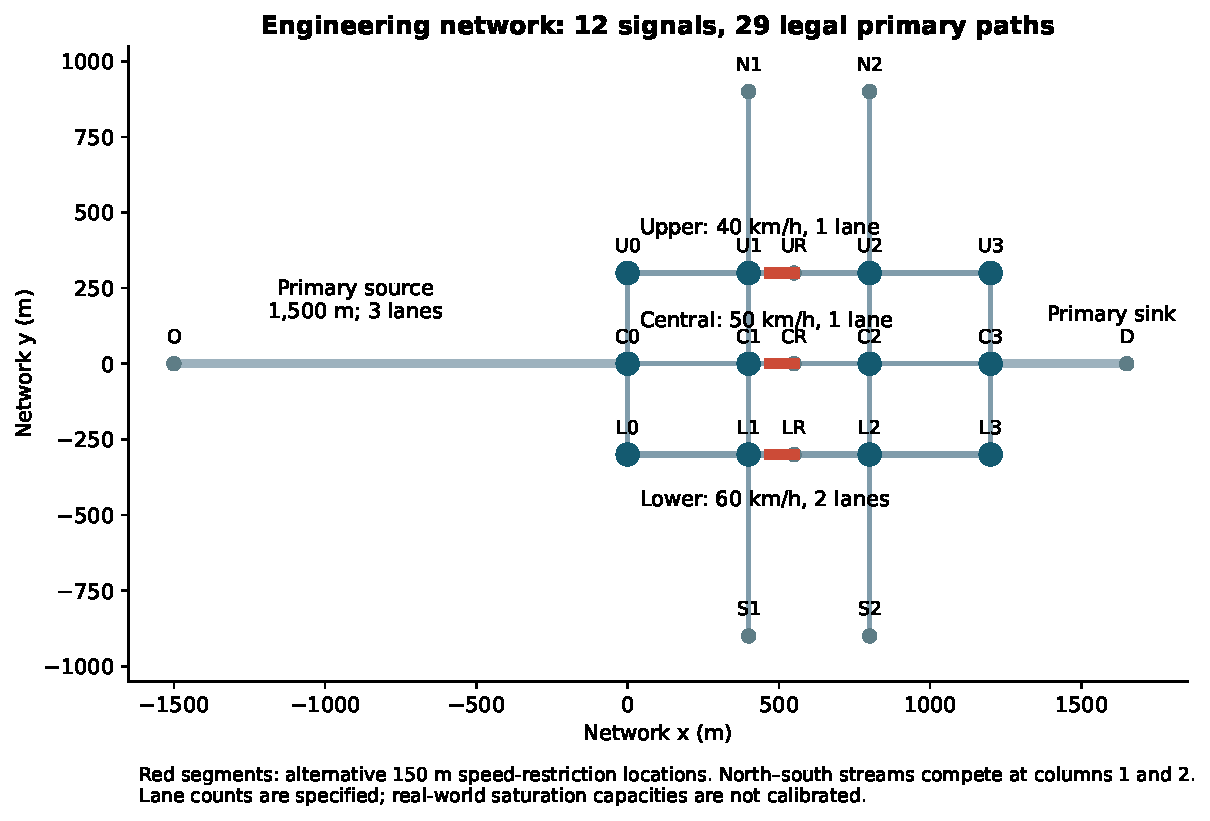
\includegraphics[width=.92\linewidth]{figures/network.pdf}
\caption{Development network. Alternative restriction sites and competing background streams permit interacting route mechanisms.}\label{fig:network}
\end{figure}

The 24 contexts are the full factorial of primary demand $\{720,1200,1680\}$\,veh/h, restriction location $\{$none, upper, central, lower$\}$ at speed ratio 0.35, and the two signal regimes. Four background streams carry 200\,veh/h each. Each context was run under six policy settings with paired seeds 8101--8103, giving 432 completed runs. SUMO 1.25.0 was used with 1\,s steps and a homogeneous HBEFA3/PC\_G\_EU4 fleet; warm-up is 600\,s, requests stop at 2400\,s, restrictions act over 600--1200\,s, teleports are disabled. All 432 runs completed with no missing vehicles, collisions or teleports.

Let $\mathcal P$ be the 29 legal paths and $L(p)$, $\widehat T_t(p)$, $\widehat E_t(p)$ denote distance, estimated in-network time and estimated grams of \CO. The policies are
\begin{align}
p_{\mathrm{SP}}&\in\arg\min_{p\in\mathcal P}L(p), &
p_{\mathrm{DTT}}&\in\arg\min_{p\in\mathcal P}\widehat T_t(p),\\
p_{\mathrm{ECO}}&\in\arg\min_{p\in\mathcal P}\widehat E_t(p), &
p_{\mathrm{TECO}}&\in\arg\min_{p:\widehat T_t(p)\le(1+\alpha)\min_q\widehat T_t(q)}\widehat E_t(p),
\end{align}
with $\alpha\in\{5,10,15\}\%$. These are our notation and finite-candidate implementation of established objectives \cite{dijkstra1959note,boriboonsomsin2012ecorouting,zeng2017svm,huang2018ecorouting}; the hard TECO filter is a disclosed adaptation of Huang's soft formulation.

\textbf{Decision-time information.} What each policy may observe, and when, is fixed and identical across policies, so that differences in outcome are attributable to the objective rather than to an information advantage. All policies share the same demand manifest, signal plans, fleet and path catalogue $\mathcal P$. SP uses only static link lengths and is therefore constant within a context. DTT and the TECO variants read link travel-time and emission estimates aggregated over \emph{completed} 60\,s intervals, so the estimate available to a vehicle requesting a route at time $t$ summarises the interval ending at or before $t$ and never contains information from the vehicle's own trip or from any later interval. Each vehicle is assigned one route at its request time and does not reroute en route; compliance is complete, so the assigned route is the driven route. The consequence for interpretation is that our policies are \emph{pre-trip} planners under lagged information, not en-route controllers: results here bound what can be achieved by choosing an objective at departure, and say nothing about mid-trip adaptation.

\textbf{Final portfolio.} Section~\ref{sec:controls} reports that ECO is outcome-identical to SP in 21 of 24 contexts and that its estimator fails route-order validation. ECO is therefore excluded from the adaptive portfolio on evidence, leaving $\mathcal A=\{\mathrm{SP},\mathrm{DTT},\mathrm{TECO}10\}$. The excluded settings are retained as controls, not discarded.

\subsection{Criteria and the definition of ``preferred''}
The estimand is the guided primary-OD cohort requested over 600--2400\,s and followed to arrival. Journey time is duration plus insertion delay; emissions are accumulated in-network tailpipe \CO. Criterion means are averaged within run, then equally across the three replications. For criterion means $y_{sak}$, positive common references $a_k$ and weights $w_k\ge0$ summing to one,
\begin{equation}
C_{sa}(w)=\sum_k w_k\frac{y_{sak}}{a_k},\qquad
R_{sa}=C_{sa}-\min_b C_{sb},
\label{eq:cost}
\end{equation}
the first being our fixed-reference linear adaptation of additive value \cite{keeney1993decisions} and the second opportunity loss \cite{kouvelis1997robust}. Lower is preferred. References are the equal mean over the $24\times3$ portfolio cells: 542.844\,s and 1263.515\,g. The primary profile is balanced, $w=(0.5,0.5)$ over time and \CO.

\textbf{Measurement definitions.} Journey time is arrival minus requested departure and therefore includes any delay before the vehicle can enter the network; emissions are accumulated in-network tailpipe \CO\ and therefore exclude idling before insertion. The two boundaries differ, which matters at high demand, and Section~4.5 reports the consequence. Fuel is excluded as a separate criterion after confirming near-proportionality to \CO\ (ratio $\approx3.135$, trip correlation $>0.999999997$) for this homogeneous fleet: retaining it would duplicate an existing criterion rather than add a decision dimension.

\textbf{Four distinct objects.} The analysis compares four things that are easily conflated, so we name them separately. Write $C^*_s=\min_{a\in\mathcal A}C_{sa}$ for the cost of the best policy \emph{observed in context $s$}, and for any selection rule $\pi$ mapping contexts to policies,
\begin{equation}
R_s(\pi)=C_{s,\pi(s)}-C^*_s \;\ge\; 0 .
\label{eq:regret}
\end{equation}
Then: (i) the \emph{best observed policy in a context}, $\arg\min_a C_{sa}$, is a per-context label, not a rule; (ii) a \emph{fixed strategy} $\pi_F(s)\equiv a_F$ ignores context and is deployable without any prediction; (iii) the \emph{hindsight best-policy benchmark} $\pi_{\mathrm{HB}}(s)=\arg\min_a C_{sa}$ attains $R_s=0$ by construction but requires every policy's realised outcome in $s$ to be known before choosing, so it is retrospective and \textbf{not deployable}; (iv) the \emph{adaptive selector} $\pi_{\widehat{}}$ attempts to approximate (iii) from pre-decision context alone, observing no policy outcome in $s$ at deployment time.

The hindsight benchmark is an upper bound on what any selector could achieve on this benchmark, in the sense of the Virtual Best Solver \cite{bischl2016aslib}. It is not an algorithm, not a routing method, and not a multi-criteria method; it exists only to normalise the others. Accordingly, \emph{available headroom} against a fixed policy $a_F$ is
\begin{equation}
H_s=C_{s,a_F}-C^*_s ,\qquad \bar H=\tfrac1{|\mathcal S|}\textstyle\sum_s H_s ,
\label{eq:headroom}
\end{equation}
and the \emph{fraction of headroom captured} by a selector is $\big(\bar H-\overline{R(\pi_{\widehat{}})}\big)/\bar H$. This quantity is bounded above by 1 (attained only by the retrospective benchmark) and is negative when the selector is worse than the fixed policy it replaces.

\subsection{Selector and evaluation protocol}
The selector predicts \emph{policy outcomes} from pre-decision context and then applies the same frozen preference model to the predictions; it never predicts a policy label directly. This ordering has two consequences we rely on: a single fitted model serves any declared weight vector without refitting, and the physical prediction is never contaminated by the preference model, so a change of weights cannot be mistaken for a change in predicted traffic behaviour.

\textbf{Features and leakage control.} Features are the scheduled primary demand, the planned restriction location and its speed ratio, and the signal regime. Each is a planning quantity fixed before the episode begins: demand comes from the scheduled manifest, restrictions are announced controls rather than unannounced incidents, and the signal regime is the controller plan. No realised outcome --- no travel time, emission, queue or flow --- enters the features. Four further controls are applied. The tree is refit from scratch on each fold. The reference scales $a_k$ in Eq.~\eqref{eq:cost} are recomputed from the training contexts of that fold only, so no test-context outcome influences the cost geometry used to choose. All three replications of a context move together between train and test, so no seed of a context can inform a decision about another seed of the same context. And no protocol result was used to select features, model settings, scaling or comparators: the settings below were fixed before the evaluations were run, and the sweep in Section~4.6 is reported for completeness rather than used for selection.

The model is a multi-output regression tree \cite{breiman2017cart} of depth 3 with minimum leaf 2, predicting training-scaled time and \CO\ for each policy. Depth 3 and leaf 8 were pre-registered for a planned 84-context training set; leaf size was rescaled to the 23-context training folds used here ($8/84\rightarrow2/23$) and no other setting was varied for the reported result. Section~\ref{sec:robust} reports the full hyperparameter sweep.

\textbf{Five distinct quantities.} Because the results report several numbers that are easy to conflate, we fix their meanings here. \emph{Prediction error} (MAE, RMSE) measures how closely predicted policy outcomes match observed ones, in seconds and grams. \emph{Ranking accuracy} counts contexts in which the predicted ordering of policies matches the observed ordering, either for the top-ranked policy or for the full ordering; it is unitless and ignores magnitudes. \emph{Decision regret} $R_s(\pi)$ of Eq.~\eqref{eq:regret} is the excess cost incurred in context $s$ by the policy the rule selected, in common cost units. \emph{Available headroom} $\bar H$ of Eq.~\eqref{eq:headroom} is the mean regret of the best fixed policy --- the total amount any selector could win. \emph{Fraction of headroom captured} is $(\bar H-\overline{R(\pi)})/\bar H$, a dimensionless ratio of the two preceding quantities. Only the last is ever quoted as a percentage of headroom in this paper, and it is never a percentage of travel time, emissions, prediction error or feature importance.

\textbf{Evaluation protocols.} With 24 contexts, the primary protocol is leave-one-context-out (LOCO): for each context the model and scales are refit on the remaining 23, and the withheld context is scored against its observed outcomes. LOCO is chosen for this design size because a single held-out split of 24 contexts would leave either too few training contexts to fit or too few test contexts to measure; it is standard for small benchmark suites in the algorithm-selection literature. Its known cost is that the 24 test decisions are not independent --- neighbouring folds share 22 of 23 training contexts --- so LOCO estimates the decision quality of the \emph{procedure} at this sample size and is optimistic relative to a single large untouched test set. We state this rather than claim a confirmatory test we do not have.

Three further protocols probe different generalisation questions. Leave-one-restriction-out withholds all six contexts sharing a restriction configuration and asks whether the selector generalises to an unseen restriction layout. A two-fold interleaved split halves the training data and measures sensitivity to training-set size. Leave-one-\emph{demand}-out withholds an entire demand level and asks the selector to extrapolate to a regime never observed; this is a deliberate stress test of the operating domain rather than a claim about expected performance, and we report it as such.

\section{Results}
\subsection{Regime structure of policy preference}\label{sec:regime}
Define the switching margin $m_s=C_{s,\mathrm{SP}}-C_{s,\mathrm{DTT}}$; negative values mean SP is preferred. Table~\ref{tab:margin} and Figure~\ref{fig:regime}(a) show that $m_s$ is negative in all eight low-demand contexts, positive in all eight high-demand contexts, and increases monotonically with demand in every cell.

\begin{table}[htbp]\centering\small
\caption{Switching margin $m=C_{\mathrm{SP}}-C_{\mathrm{DTT}}$ in common cost units. Negative: SP preferred. The sign change is bracketed by the demand grid, not localised within it.}\label{tab:margin}
\begin{tabular}{llrrrc}\toprule
Signal & Restriction & $q=720$ & $q=1200$ & $q=1680$ & Crossing bracket (veh/h)\\\midrule
Balanced & none    & $-0.0551$ & $0.4204$ & $1.0139$ & $(720,1200]$\\
Balanced & upper   & $-0.0515$ & $0.4382$ & $0.9418$ & $(720,1200]$\\
Balanced & central & $-0.0195$ & $0.8056$ & $1.1137$ & $(720,1200]$\\
Balanced & lower   & $-0.0562$ & $0.4196$ & $1.0134$ & $(720,1200]$\\\midrule
Arterial & none    & $-0.0184$ & $-0.1269$ & $0.3249$ & $(1200,1680]$\\
Arterial & upper   & $-0.0198$ & $-0.1318$ & $0.3165$ & $(1200,1680]$\\
Arterial & central & $-0.0423$ & $0.0488$ & $0.3893$ & $(720,1200]$\\
Arterial & lower   & $-0.0110$ & $-0.0954$ & $0.2952$ & $(1200,1680]$\\
\bottomrule\end{tabular}\end{table}

\textbf{Three regimes.} The 24 contexts separate into three qualitatively different operating regions, and the distinction organises every later result.

\emph{(A) Low-demand regime ($q=720$).} The margin is negative in all eight cells and small in magnitude ($-0.011$ to $-0.056$). Congestion is light enough that the shortest path is also close to the fastest, so minimising distance and minimising estimated time nearly coincide; SP wins because it achieves essentially the same time over a shorter distance, and hence lower emissions. Decisions here are easy but also cheap to get wrong: the worst available policy costs only 0.0342 mean regret.

\emph{(B) Transition regime ($q=1200$).} This is the only region where the two signal regimes disagree, where the margin is small relative to its seed-to-seed variation, and where policy identity genuinely depends on the full context rather than on demand alone. All four contexts whose winner is unstable across seeds lie at $q=1200$ or immediately below it; all three held-out selector errors lie here (Section~4.2); and the mean regret of the worst policy rises tenfold to 0.3229. The transition regime is where the decision problem actually lives.

\emph{(C) High-demand regime ($q=1680$).} The margin is large and positive in all eight cells ($+0.295$ to $+1.114$), DTT is best in every context, and the penalty for the wrong choice is severe (0.6761 for the worst policy; fixed SP alone incurs 0.676). In these eight contexts congestion on the shortest path is heavy enough that the time-based policy is preferred under every restriction and signal configuration tested. Decisions here are easy again, but expensive to get wrong.

The outer regimes are easy for different reasons and the transition regime is hard for one reason: it is where the ordering of two established objectives is genuinely contested.

\textbf{The signal regime displaces the transition.} Under balanced timing every cell has already crossed by 1200\,veh/h (mean margin $+0.521$); under arterial timing three of four cells have not (mean margin $-0.076$) and cross only by 1680\,veh/h. Arterial-priority timing therefore raises the demand at which adapting the policy begins to pay by at least one grid step. The central-restriction cell crosses earlier than its siblings under both regimes, which indicates an interaction between restriction placement and the crossing point that the present grid cannot resolve further.

The operational reading is that \emph{demand alone is not sufficient to characterise which policy is preferable}. A rule calibrated under one signal-timing plan would misclassify contexts under the other across an interval of at least 480\,veh/h --- the whole of the region where the two regimes disagree. Any deployment that selects a routing policy from traffic state must therefore treat the signalisation plan as part of the context, not as a fixed background condition.

We deliberately do not assert a mechanism. The experiment varies the green split between competing directions, which changes the delay experienced on the alternative corridors and hence their relative attractiveness, and the observed displacement is consistent with that explanation; but the experiment does not isolate it from other consequences of the timing change, and no mechanism-separating condition was run. We therefore report the displacement as an observed interaction and leave its cause open.

\begin{figure}[htbp]\centering
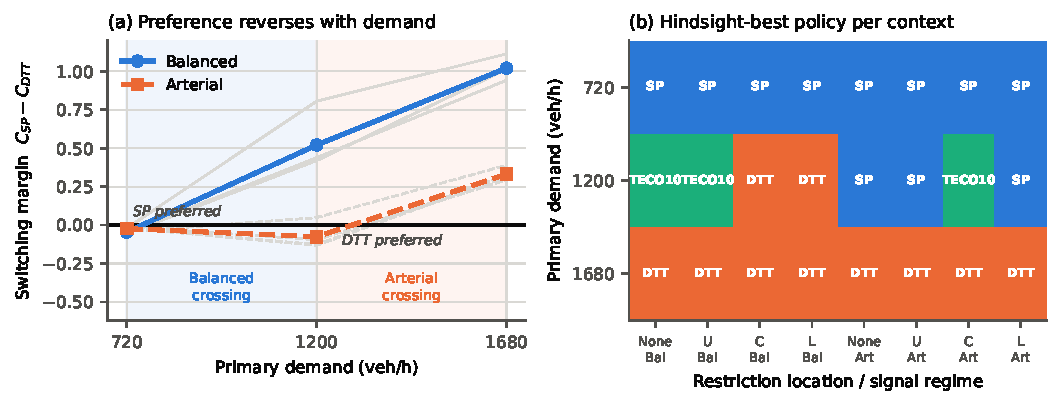
\includegraphics[width=\linewidth]{figures/regime_structure.pdf}
\caption{(a) The switching margin reverses sign with demand; heavy lines are the mean over restriction locations, faint lines the individual cells. Shading marks the bracketing intervals, not estimated crossing points. (b) Hindsight-best policy in each of the 24 contexts.}\label{fig:regime}
\end{figure}

\textbf{Is the change abrupt or gradual?} The increment of the margin grows with demand in seven of the eight cells, so the crossing accelerates rather than jumping. The margin is monotone in demand in five of eight cells: in the three arterial cells with no, upper or lower restriction it \emph{decreases} from 720 to 1200\,veh/h (by $-0.084$ to $-0.112$) before rising sharply, so under arterial priority SP's advantage first strengthens at moderate demand and only then collapses. The reversal is thus not a uniform drift in one direction, and a two-point characterisation of it would be misleading. Seed dispersion follows the same pattern: the standard deviation of $m$ across the three seeds is 0.003--0.038 at 720 and 1680\,veh/h but 0.018--0.121 at 1200\,veh/h, largest precisely where the margin is smallest. We emphasise what the design cannot support: with demand levels 480\,veh/h apart, the crossing is \emph{bracketed} to intervals of that width and is not localised. We therefore report brackets throughout and make no point estimate of a switching threshold. Section~\ref{sec:future} specifies the minimal experiment that would localise it.

\textbf{What changes across the regimes.} The reversal is the crossing of a fixed structural penalty against a growing congestion penalty, and both terms are observable in the completed runs. DTT's chosen routes are consistently about 8\% longer than the shortest path, and that penalty is almost constant across regimes: the SP$-$DTT distance difference is $-250$, $-288$ and $-277$\,m at 720, 1200 and 1680\,veh/h. What changes is the cost of using the shorter corridor. Implied in-network mean speed falls from 37.80 to 18.31\,km/h for SP ($-51.6\%$) but only from 38.43 to 23.80\,km/h for DTT ($-38.1\%$); stopped vehicle-time per vehicle rises from 176.1 to 436.8\,veh-s for SP against 169.7 to 322.5 for DTT; and emission intensity rises from 255.1 to 590.7\,g/km for SP against 248.5 to 423.2\,g/km for DTT. Consequently the SP$-$DTT in-network time difference moves from $-17.9$\,s at low demand to $+113.7$\,s at high demand, and the \CO\ difference from $-44.7$ to $+416.9$\,g.

The decomposition is therefore consistent with the following reading, which we state as an interpretation rather than an identified mechanism. At low demand the two policies achieve nearly the same speed (a $1.6\%$ difference) and nearly the same queueing, so the detour buys almost no congestion relief and is not compensated: SP wins on both criteria simultaneously. As demand rises the shortest corridor degrades faster than the alternatives, and once the accumulated congestion penalty exceeds the fixed distance penalty the sign of the margin flips. The experiment does not isolate this mechanism from other consequences of raising demand, and the available outputs do not contain per-vehicle route shares or per-signal exposure measures, so we do not claim causal identification.

\textbf{Cost of getting it wrong.} The penalty for a fixed policy grows sharply with demand. Mean regret of the worst available policy is 0.0342 at 720\,veh/h, 0.3229 at 1200\,veh/h and 0.6761 at 1680\,veh/h.

\textbf{Seed stability.} The hindsight-best policy is identical across all three seeds in 20 of 24 contexts, and the sign of the switching margin is stable in 22 of 24. The four unstable contexts are D005 and the three balanced-signal contexts at 1200\,veh/h --- that is, the instability sits inside the transition band, which is where ties are expected, and does not affect the low- or high-demand regimes.

\subsection{Decision headroom and held-out selection}
Fixing DTT is the best single policy but is not optimal everywhere: it leaves 0.03018 mean and 0.13176 maximum regret, and is beaten in 14 of 24 contexts. Table~\ref{tab:decision} gives the decision outcome.

\begin{table}[htbp]\centering\small
\caption{Decision quality under the balanced profile. The selector is evaluated leave-one-context-out; the hindsight benchmark is not deployable.}\label{tab:decision}
\begin{tabular}{lrrcc}\toprule
Method & Mean regret & Max regret & Optimal & Within 1\% \\\midrule
Fixed SP & 0.31825 & 1.11368 & 11/24 & 11/24 \\
Fixed DTT (best fixed) & 0.03018 & 0.13176 & 10/24 & 11/24 \\
Fixed TECO10 & 0.20757 & 1.01394 & 9/24 & 9/24 \\
\textbf{Adaptive selector (held-out)} & \textbf{0.00606} & \textbf{0.11545} & \textbf{21/24} & \textbf{22/24} \\
Hindsight best-policy benchmark & 0.00000 & 0.00000 & 24/24 & 24/24 \\
\bottomrule\end{tabular}\end{table}

\textbf{Where the headroom is.} Decomposing the same quantities by regime localises the decision opportunity sharply. Mean regret of fixed DTT is 0.03422 at low demand, 0.05633 in the transition band and \emph{exactly zero} at high demand, so regimes A and B hold $37.8\%$ and $62.2\%$ of the total headroom respectively and regime C holds none: DTT is optimal in all eight high-demand contexts and there is nothing for adaptation to win there. The penalty at high demand is for using the \emph{wrong fixed} policy --- fixed SP incurs 0.67611 --- not for failing to adapt. The held-out selector attains zero mean regret in both outer regimes and carries all of its residual regret (0.01818) in the transition band. Adaptation is therefore worth having in exactly the two regimes where a single fixed policy is not already optimal, which is a stronger and more specific statement than an aggregate figure conveys.

\textbf{Reading the ladder.} The three fixed rows and the benchmark row bound the problem. Fixed SP is a poor policy overall (0.31825) but optimal in 11 contexts --- all of them low-demand --- which is precisely the regime structure of Section~4.1 seen from the decision side. Fixed DTT is the best single choice, and its 0.03018 mean regret is the quantity an adaptive method must beat: it is the \emph{available headroom} $\bar H$ of Eq.~\eqref{eq:headroom}. It is not spread evenly; DTT is already optimal in 10 contexts and is beatable in 14.

\textbf{What 79.9\% does and does not mean.} The selector's mean regret is 0.00606 against $\bar H=0.03018$, so
\[
\frac{\bar H-\overline{R(\pi_{\widehat{}})}}{\bar H}=\frac{0.03018-0.00606}{0.03018}=0.799 .
\]
This is \emph{the fraction of the available decision headroom captured relative to the best fixed baseline} --- that is, of the gap between fixing DTT and the retrospective benchmark, the selector closes about four fifths. It is \textbf{not} a 79.9\% improvement in travel time, emissions or any physical quantity, and we avoid that phrasing throughout. In physical terms the same comparison is modest: averaged over the 24 contexts the selector's chosen policies realise 412.17\,s and 1114.64\,g per vehicle against 425.17\,s and 1145.36\,g for fixed DTT, a reduction of 13.00\,s ($3.06\%$) and 30.71\,g ($2.68\%$); restricted to the 14 contexts where DTT is not already optimal the reduction is 22.28\,s and 52.65\,g. Readers should judge the result on those magnitudes as well as on the normalised fraction.

Two further qualifications bound the claim. The percentage is defined against a \emph{finite benchmark}: both $\bar H$ and the hindsight reference are properties of these 24 contexts, and a different context grid would yield a different denominator, so the figure is not a transferable constant and certainly not evidence of a deployment benefit in a real city. And it is a LOCO estimate, which as noted in Section~3.3 is optimistic relative to a single untouched test set.

\textbf{Prediction versus decision.} Out-of-sample prediction error is 44.63\,s MAE (79.73\,s RMSE) on journey time and 82.38\,g MAE (122.09\,g RMSE) on \CO, i.e.\ 8.2\% and 6.5\% of the respective means. The selector is thus far from an accurate simulator of policy outcomes, yet recovers most of the decision value --- the two quantities are not interchangeable \cite{elmachtoub2022smart}, and a selector needs only to order policies correctly, not to predict them precisely.

\textbf{What the selector actually learned.} Inspecting the fitted tree, the root split is on demand at 1440\,veh/h, isolating the high-demand regime; the second level splits on signal regime in both branches; and a further demand split at 960\,veh/h separates the low-demand from the transition contexts. Only two of the six features carry any importance --- demand ($74.6\%$) and signal regime ($25.4\%$) --- and the four restriction-location indicators are never used, which is consistent with leave-one-restriction-out reproducing the LOCO outcome exactly. The learned structure is thus a direct encoding of the regime map of Section~\ref{sec:regime}.

This bears on whether the selector is merely a demand classifier, and the honest answer is that it largely is. Holding the evaluation fixed and varying only the model, headroom capture is $53.1\%$ at depth 1 (a single split, on demand at 1440\,veh/h), $52.8\%$ at depth 2 --- which adds the signal split and gains nothing --- and $79.9\%$ at depth 3, where a \emph{second demand split} at 960\,veh/h finally separates the low-demand from the transition contexts. The step from 53.1\% to 79.9\% is therefore attributable to resolving demand more finely, not to adding the signal feature. Ablating the signal feature altogether at depth 3 gives $72.9\%$ against $79.9\%$ with it, so conditioning on the signalisation plan is worth about $7$ percentage points of headroom capture: a real but secondary contribution on top of a predominantly demand-driven rule. We note this explicitly because the tree's \emph{feature importance} --- $25.4\%$ for signal regime --- is a variance-reduction share in the fitted regression and is not a decision-side quantity; it should not be read as the signal regime supplying a quarter of the recovered decision value.

\textbf{Prediction, ranking and decision are three different things.} Classifying every held-out context by where its error first appears separates them empirically. In 18 of 24 contexts the prediction is imperfect (mean relative error $5.9\%$) yet the top-ranked policy is still correct and regret is zero. In 3 contexts the ranking changes but the affected policies are outcome-equivalent, so regret remains zero. In 3 contexts the ranking changes and regret is substantial (mean 0.04847, maximum 0.11545). The full three-policy ranking is exactly right in only 10 of 24 contexts, the top-ranked policy in 18, and the decision incurs zero regret in 21 --- decision quality exceeds top-1 ranking quality, which exceeds full ranking quality, which exceeds prediction quality. Two contexts illustrate the endpoints: D021 has a $24.4\%$ mean prediction error and zero regret, while D014 has an $18.2\%$ error that flips the ranking and costs 0.11545. This is the predict-then-optimise distinction \cite{elmachtoub2022smart} exhibited on our own data rather than asserted.

\textbf{Where the errors are.} All three residual errors lie in the transition regime: the selector is optimal in 8/8 low-demand and 8/8 high-demand contexts and errs only at 1200\,veh/h (D009, D011 and D014, the last contributing the 0.11545 maximum). Region (B) of Section~4.1 is therefore simultaneously where the decision matters, where seeds disagree, and where the selector fails --- three independent symptoms of the same underlying property, that the ordering of the two objectives is genuinely contested there. Leave-one-restriction-out reproduces the LOCO decision outcome exactly, so generalisation across restriction layouts is not the difficulty; the two-fold interleaved split, with half the training data, captures 14.8\%, indicating that training-set coverage rather than model form is the limiting factor.

\subsection{The extrapolation boundary}
Withholding an entire demand level reverses the conclusion (Figure~\ref{fig:decision}(b)). Pooled over the three folds the selector incurs 0.07649 mean regret against 0.03018 for the best fixed policy. Holding out 1680\,veh/h is the clearest failure: DTT is optimal in all eight contexts, yet the selector trained only on 720 and 1200\,veh/h chooses DTT or TECO10 and incurs 0.14856 mean regret where fixing DTT would incur none.

\begin{figure}[htbp]\centering
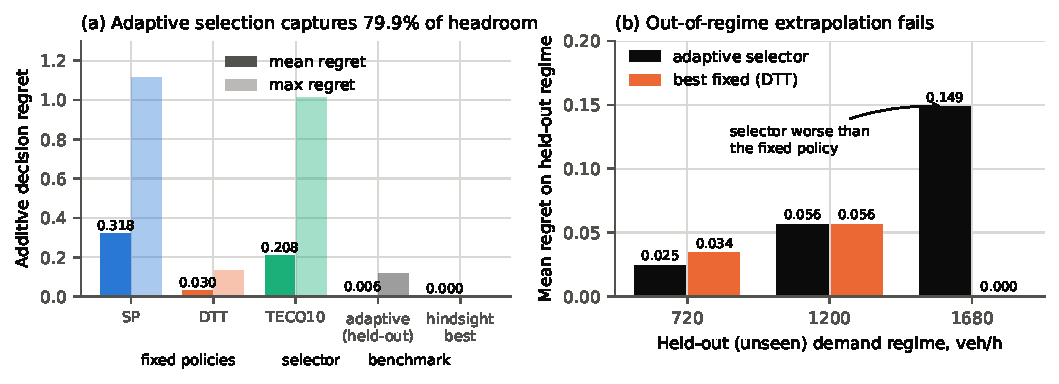
\includegraphics[width=\linewidth]{figures/decision_outcome.pdf}
\caption{(a) Decision quality of fixed policies, the held-out selector and the hindsight benchmark. (b) Holding out an entire demand regime: the selector becomes worse than the best fixed policy.}\label{fig:decision}
\end{figure}

The three folds are not three instances of one phenomenon: they occupy different positions relative to the training support, and behave differently. Withholding 1200\,veh/h leaves the test point \emph{inside} the support, in the gap between 720 and 1680; the selector then chooses DTT in all eight contexts and reproduces fixed DTT exactly (0.05633 for both), gaining nothing and losing nothing, because with only the outer regimes in training the tree learns no distinction that applies in between. Withholding 720\,veh/h places the test point \emph{below} the support; the selector, never having seen a regime in which SP wins, chooses DTT or TECO10 throughout and misses the optimum in all eight contexts --- SP would have incurred zero regret --- although it still edges fixed DTT (0.02456 against 0.03422) because DTT is a poor choice at low demand too. Withholding 1680\,veh/h places the test point \emph{above} the support, and this is the damaging case: DTT is optimal in all eight withheld contexts so fixed DTT incurs zero regret, while the selector extrapolates its partition and assigns TECO10 to half the region, incurring 0.14856.

Interpolation into a covered gap is therefore safe but uninformative, whereas extrapolation beyond the support is where thedamage occurs, and it is worst above the highest observed demand.

The asymmetry matters for deployment. A fixed policy has a property the selector lacks: its regret is bounded by how badly that one policy performs, and cannot be inflated by the selector confidently applying a rule learned elsewhere. When the operating domain is exceeded, the selector's errors are not merely uninformed but systematically wrong, because a tree extrapolates by extending the partition it already has rather than by abstaining. This is the practical boundary of the method: within the observed regime span adaptation is reliable and worthwhile; outside it, the fixed policy is the safer choice.

The requirement is therefore coverage of the regime-defining factors rather than model capacity. A depth-1 tree --- a single split on demand --- already captures 53.1\% of the headroom (Section~\ref{sec:robust}), so the available decision value is not gated by model expressiveness. What gates it is whether the demand levels and signal plans encountered in service were represented when the selector was fitted. For an operator this converts a modelling question into an instrumentation and monitoring question: characterise the regimes the system will meet, verify that they lie inside the fitted domain, and fall back to a fixed policy when they do not.

\subsection{Negative controls}\label{sec:controls}
\textbf{The environmental objective was not a distinct policy.} ECO is outcome-identical to SP --- in time, \CO, distance and P95 to machine precision --- in 21 of 24 contexts. Its decision-time estimator passes accounting and aggregate prediction yet fails route ordering: maximum edge/trip mass discrepancy is 0.16945\% and native per-vehicle algebra error $6.945\times10^{-7}$; over 270{,}432 matched primary trips, selected-path \CO\ forecasts give WAPE 14.71\% with signed bias $-0.315\%$, improving on a frozen 600\,s snapshot (22.38\%) and a warm-up emissions-per-metre baseline (36.88\%). But in a 232-run fixed-replay probe over eight context--seed panels, in which only one tagged vehicle's route varies, the median rank correlation is 0.536 and the mean relative emission selection loss is 21.62\% against a declared 10\% screen, with a 78.16\% maximum and the predicted-best route matching the observed best in only 3 of 8 panels (Figure~\ref{fig:eco}). Good average prediction over previously selected routes did not confer correct ranking near the predicted optimum. ECO was therefore removed from the adaptive portfolio: in this environment it supplied no independent environmental decision dimension. We do not conclude that eco-routing is ineffective in general, only that this estimator in this environment did not support a distinct policy.

\begin{figure}[htbp]\centering
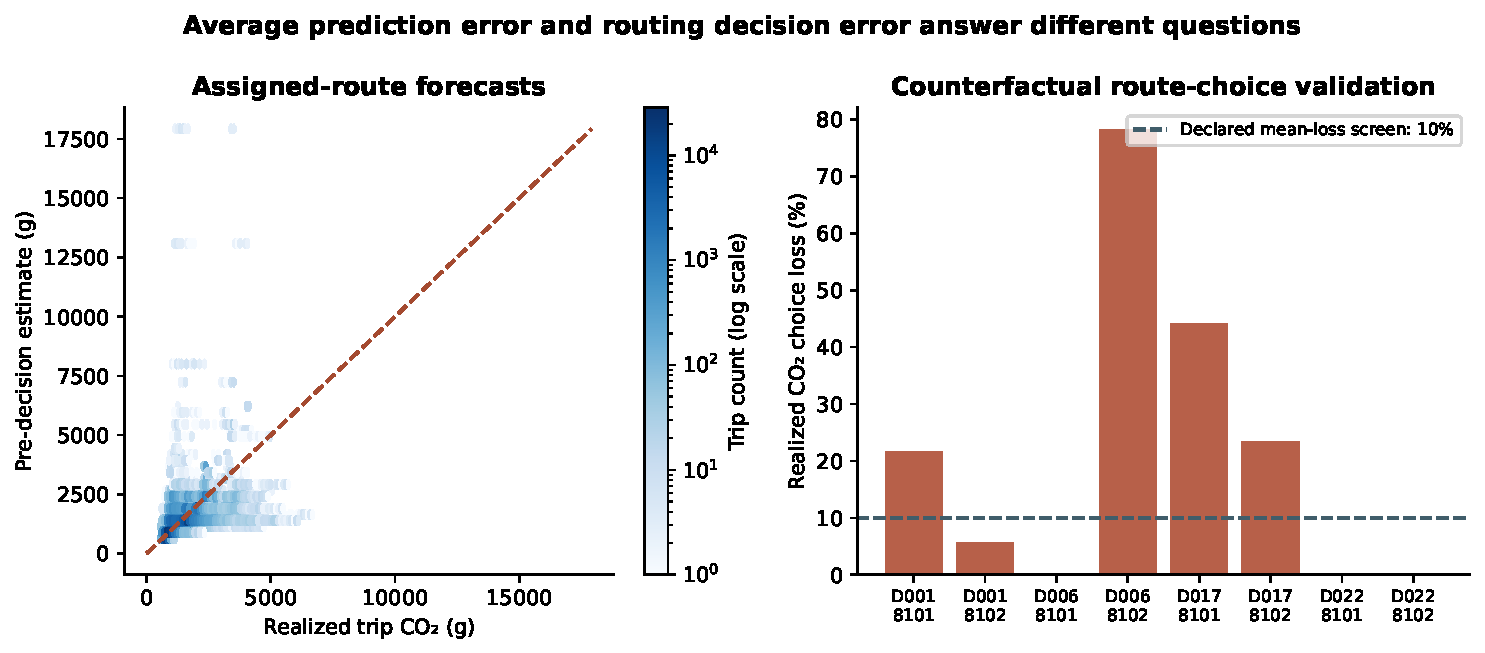
\includegraphics[width=\linewidth]{figures/forecast_and_decision.pdf}
\caption{Aggregate forecast accuracy and marginal route-choice validity are distinct. The right panel covers eight context--seed panels, not 232 independent contexts.}\label{fig:eco}
\end{figure}

\textbf{The preference layer changes no decision.} Time and \CO\ are strongly aligned in this environment (pooled Spearman 0.982). Repeating the full held-out evaluation at $w_{\text{time}}\in\{0,0.25,0.5,0.75,1\}$ --- that is, from a purely time-oriented preference to a purely emissions-oriented one --- leaves every one of the 24 selector decisions unchanged, and the hindsight-optimal label changes in exactly one context (D011, and only at the pure-emissions extreme).

This has a positive and a negative reading, and both are findings rather than defects. Positively, it is the strongest available evidence that the regime structure of Section~\ref{sec:regime} is \emph{not an artefact of the declared weights}. Sweeping $w_{\text{time}}$ over 21 values in steps of 0.05 from 0 to 1, SP is the hindsight-best policy in \emph{every} low-demand context and DTT in \emph{every} high-demand context at \emph{every} weighting, with no exception; the sign pattern of the switching margin across the eight transition contexts is likewise identical at all tested profiles. A reviewer suspecting that the winners were manufactured by a weight choice can be answered directly --- no weight in the admissible range produces a different set of selector decisions, and none breaks the regime structure. Negatively, it means the multi-criteria layer here \emph{defines} preference without \emph{discriminating} between policies: in this benchmark, with these two criteria, it is doing formal rather than empirical work.

The correct response is to report this, not to add further preference methods. Applying TOPSIS, VIKOR, PROMETHEE or a fuzzy variant to two criteria correlated at 0.982 would produce agreement by construction and would misrepresent methodological agreement as validation. We therefore retain one transparent additive formulation, state plainly that it is nearly inert in this environment, and make no claim for the decision model as a contribution. Whether a genuinely independent second criterion would restore discrimination is an open question that this benchmark cannot answer, because it does not contain one.

\textbf{TECO applies its constraint correctly.} Realised journey time exceeds the $(1+\alpha)$ bound in 54.1\%, 35.6\% and 26.1\% of within-run trips for $\alpha=5,10,15\%$. The constraint is imposed on the \emph{estimated} pre-decision travel time, and these shares compare a realised duration with a predicted benchmark. This is a forecast-to-realised mismatch, not a violation of the algorithm's own constraint. We did not re-audit the implementation source in this study and make no claim beyond the observed shares.

\subsection{Robustness}\label{sec:robust}
\textbf{Hyperparameters.} Across tree depths $\{1,2,3,4,\text{unlimited}\}\times$ leaf sizes $\{1,2,3\}$, headroom capture ranges from 50.9\% to 79.9\% and is positive in all 15 settings. Depth 1 --- a single split on demand --- already captures 53.1\%, confirming that the result rests on regime structure rather than model flexibility.

\textbf{Seeds.} Training on two seed blocks and scoring against the withheld third gives 60.8\%, 67.7\% and 90.2\% capture; the gain is not a replication artefact.

\textbf{Scaling.} Recomputing the evaluation with training-only reference scales rather than common scales gives 79.8\%, so the fold-wise scaling choice does not drive the result.

\textbf{Measurement boundary.} Journey time includes insertion delay while in-network \CO\ excludes pre-insertion idling, and insertion delay is large and strongly policy-dependent at high demand (mean 0.12, 5.54 and 262.41\,s at 720, 1200 and 1680\,veh/h; 810.29\,s in the worst run; 447.5\,s for SP against 6.3\,s for DTT at 1680\,veh/h). Recomputing every decision on in-network time alone changes the preferred policy in \emph{none} of the 24 contexts, and mean headroom only from 0.03018 to 0.03281. The regime structure is therefore not an artefact of the emission accounting boundary, although absolute journey times at high demand clearly are affected by it.

\textbf{Preserved pilot.} An earlier completed 270-run pilot over 30 contexts with SP, DTT and a time-dependent variant gives SP 241.050\,s/639.364\,g, DTT 200.261\,s/506.551\,g and TDR 205.194\,s/523.213\,g, with DTT lowest on both context-average criteria in all 30 contexts and therefore zero adaptive headroom. That environment exhibited no regime reversal; the present network does. The contrast is the reason regime structure must be established empirically before a selector is contemplated.

\section{Discussion}
The practically useful statement is conditional. Adapting the routing policy captures roughly four fifths of the available decision headroom when the deployment regime has been observed during fitting, and is worse than not adapting when it has not. The conditionality, not the fraction, is the result.

\textbf{Adaptation is a property of the environment, not of the algorithms.} The policies compared here are unchanged between our pilot environment, where one policy dominated all 30 contexts and adaptation was worth exactly nothing, and the present network, where it is worth 0.03018 units and 13\,s per vehicle. Nothing about SP or DTT changed; the traffic environment did. It follows that the question ``should this system adapt its routing policy?'' cannot be answered from the policies, the decision model or the learner. It is an empirical question about the demand and control regimes the system will meet, and it must be measured before an adaptive component is justified. Our pilot is the negative instance of exactly this measurement and is retained in the paper for that reason.

\textbf{A fixed policy has a safety property that the selector lacks.} Outside the observed regime span a fixed policy is not merely a baseline but the correct choice. Its regret is bounded by how badly that single policy performs across conditions, whereas the selector's regret can be inflated without limit by confidently applying a partition fitted elsewhere --- as the 1680\,veh/h fold shows, where fixed DTT is optimal and the selector is not. A deployed selector therefore needs an explicit operating domain and a fallback, and the fallback should be a fixed policy rather than a lower-confidence prediction.

\textbf{The context is not demand alone.} Because the transition is displaced by the signal regime across an interval of at least 480\,veh/h, an operator calibrating such a system must cover the signalisation plans in force as well as the demand range. A selector calibrated under one timing plan and deployed under another would be extrapolating in a dimension its designer may not have recognised as a regime variable at all. This is the practical content of the signal-regime finding: it enlarges the set of factors that must be instrumented, without requiring any change to the routing algorithms.

\textbf{Effort belongs in characterisation, not in model capacity.} A single split on demand recovers 53.1\% of the headroom and the full sweep of tree depths spans only 50.9--79.9\%. The marginal return to model sophistication on this benchmark is therefore small, while the return to knowing where the regimes change --- which our own design can only bracket to 480\,veh/h --- is large. We read this as an argument for spending experimental budget on locating transitions rather than on selectors.

\textbf{What the negative controls protect.} The environmental objective did not survive a validated route-ordering test, and the preference weights changed no decision. Reported alone, the 79.9\% figure would imply a richer multi-objective problem than this environment contains: a reader would reasonably infer a time--emissions trade-off being resolved by a preference model, when in fact the two criteria are nearly collinear and the decision is effectively one-dimensional. Keeping both controls in the paper is what makes the positive result readable at its true scope.

\section{Limitations}
We state each limitation together with the claim it prevents us from making.

\emph{One synthetic topology and one primary OD structure.} Prevents any claim that the bracket values, the 79.9\% figure or the signal displacement transfer to another network. The qualitative pattern --- that a reversal exists and is displaced by signal timing --- is demonstrated on one benchmark and is a hypothesis elsewhere. No second independent network was tested.

\emph{One vehicle class, deterministic behaviour.} Prevents claims about fleet-mix effects, about heterogeneous driver compliance, and about emissions differences arising from vehicle technology. It also makes the fuel/\CO\ redundancy a property of this fleet rather than a general result.

\emph{Twenty-four contexts and three replications.} Prevents a confirmatory held-out claim. LOCO is appropriate at this size but its folds share 22 of 23 training contexts, so it estimates procedure quality optimistically; no separate untouched test set was reserved, and we report no significance test on context-level differences.

\emph{Finite context grid, 480\,veh/h spacing.} Prevents any point estimate of a switching threshold, any statement about the shape of the margin near the crossing, and any resolution of the restriction-placement interaction visible in the central cell. We report brackets only.

\emph{Scheduled and announced restrictions.} Prevents claims about unexpected incidents. Our features are planning quantities known before the episode; a selector facing unannounced disruption would require a detection component that this study does not contain or evaluate.

\emph{Decision features assumed known and compliance complete.} Prevents claims about partial adoption, about routing advice that users decline, and about degradation when the assumed context is measured with error. Every assigned route is driven.

\emph{Pre-trip assignment with lagged information, no en-route rerouting.} Prevents any comparison with en-route adaptive control; results bound what departure-time objective selection can achieve, not what mid-trip adaptation could.

\emph{Specified rather than calibrated lane capacities.} Prevents quantitative transfer of the congestion levels at which the transition occurs to a real corridor with measured saturation flows.

\emph{Known-defective environmental estimator.} Prevents any claim about eco-routing effectiveness in either direction. We report that this estimator failed route ordering here; we do not conclude that eco-routing is ineffective, and its repair was not attempted.

\emph{Insertion-delay measurement sensitivity.} Journey time includes pre-insertion delay while in-network \CO\ excludes it. Section~\ref{sec:robust} shows no preferred policy changes under either boundary, so decision claims are unaffected; but absolute journey times at 1680\,veh/h are boundary-dependent and should not be read as corridor travel times.

\emph{Aggregated per-run outputs.} The completed runs record cohort means, not per-vehicle route shares or per-signal exposure. Prevents any causal identification of the mechanism behind the reversal or the signal displacement: we can show that SP's speed and emission intensity degrade faster than DTT's, but not attribute that degradation to specific movements or signal phases. The mechanistic reading in Section~\ref{sec:regime} is offered as a consistent decomposition only.

\emph{Analytical, non-elicited weights.} Prevents any claim that the preference profiles represent stakeholder values. Given that no weight in the admissible range changes a decision here, this limits interpretation rather than results.

\emph{Targeted, non-systematic literature audit.} Prevents any priority or novelty claim. We assert differences from named studies only.

\section{Future work: the minimal localising experiment}\label{sec:future}
The single unresolved quantity is where within each bracket the reversal occurs. Localising it does not require a large factorial. Bisecting the two brackets identified in Table~\ref{tab:margin} requires two additional demand levels --- 960\,veh/h for the balanced bracket and 1440\,veh/h for the arterial bracket --- run over the existing eight restriction/signal cells, three policies and three seeds: 144 additional simulations, roughly 1.5 minutes of compute at the throughput observed for the completed matrix. A second bisection round would halve the remaining interval for a further 144 runs. This experiment characterises the switching regime; it does not increase sample size for the selector, and the selector result above does not depend on it. We specify it here rather than report it: the simulation network, route and configuration files were not available in this session, and running a reconstructed network would have produced results not comparable with the 432 completed runs. No additional simulation was executed and none is reported.

\section{Conclusion}
In a controlled 12-signal urban mesh, the preferred established routing policy reverses with traffic demand --- shortest-distance below the reversal, dynamic travel-time above it --- and the reversal is displaced to higher demand by arterial-priority signal timing. Adapting the policy across this structure is worth 0.03018 mean regret units against the best fixed policy, of which an interpretable depth-3 tree recovers 79.9\% on held-out contexts while being optimal in 21 of 24. Applied outside the demand regimes it was trained on, the same selector is worse than the fixed policy it replaces. Adaptive routing-policy selection is governed by regime coverage of the context space, not by model capacity. An environmental objective and a multi-criteria preference layer were both tested and both found inert in this environment, and are reported as controls rather than removed from the record.

\section{Reproducibility}
Every quantity in this paper derives from the 432 completed runs and the audited project workbook. The workbook exports one row per run; a single script converts it to a flat run table, and a second recomputes every reported value into a machine-readable results file from which the tables and figures are generated. The remaining scripts correspond one-to-one with the reported analyses: regime structure and seed stability; held-out selection under the four protocols; the hyperparameter, weight, seed and scaling robustness battery; and the demand-extrapolation stress test. Re-running them reproduces every number in Tables~\ref{tab:margin} and~\ref{tab:decision} and both figures.

The reported evaluation fixes the random state of the tree, and the only stochastic element of the underlying experiment --- the demand manifest --- is controlled by the three named seeds, so the analysis is deterministic given the run table. Three sheets added to the workbook (regime transition, decision evaluation, negative controls) carry the derived values alongside the original 22 sheets, which are unmodified.

Two things are deliberately absent. The SUMO network, route and configuration files were not available to the analysis reported here, so the run table is the reproduction boundary: the analysis reproduces exactly, while regenerating the runs themselves requires the original scenario package. And the localising experiment of Section~\ref{sec:future} is specified and scripted but was not executed, for the reason given there.

\paragraph{Assistance.} AI assisted analysis, literature triage and drafting; human authors remain responsible for source verification, methodological acceptance and submission.

\bibliographystyle{unsrt}
\bibliography{references}
\end{document}
